\documentclass[../main.tex]{subfiles}
\begin{document}
	$G = (g_{ij})$ ковариантный метр. тензор\\
	$G^{-1} = (g^{ij})$ контрвариантный метр. тензор
	\begin{defin}
		$e_1 \ldots e_n$ базис $V$ евклидово пространство.
		$e^1 \ldots e^n$ незывается \underline{взаимным} для базиса $e_1 \ldots e_n$, если 
		$\boxed{(e^i, e_j) = \delta^i_j = (e_j, e^i)}\n
		e_1 \ldots e_n$ \underline{взаимный} для базиса $e^1 \ldots e^n$\n
		\underline{Взаимные базисы $e_1 \ldots e_n$ и $e^1 \ldots e^n$}
	\end{defin}
	\begin{examples}\ \\
		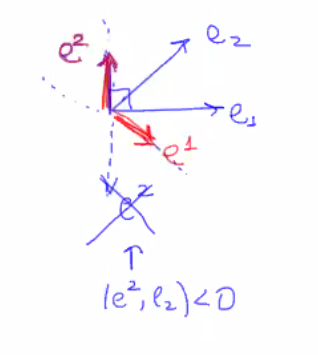
\includegraphics[width=100px]{pic15}
		$(e_i, e^j) = \delta^j_i = \left\{\begin{array}{c}
		1, i=j\\
		0, \neq j
		\end{array}\right.
		$
	\end{examples}
	\begin{theorem}
		$\forall $ базиса $e_1 \ldots e_n$ пространства $V \; \; \exists!$ взаимный базис $e^1 \ldots e^n$
	\end{theorem}
	\begin{proof}
		$e_1 \ldots e_n\n
		e^j = t^i_j e_i \; \; \; \; t^i_j \leftrightarrow T_j \; \; \; \; (e_i, e^j) = \delta^j_i \; \; \; \; \; \; \; T_{e_i \rightarrow e^j} = (T_1 \ldots T_j \ldots T_n)\n
		\Gamma = G(e_1 \ldots e_n) \; \; \; \; \; \delta^j_i = (e_i, e^j) = \underset{\stackrel{\updownarrow}{E^T_i}}{x^T} \Gamma \underset{\stackrel{\updownarrow}{T_j}}{y} \Leftrightarrow E = E\Gamma T \Leftrightarrow \underset{\stackrel{\Updownarrow}{T = \Gamma^{-1} \Rightarrow \exists! \text{ взаимный базис } e^j}}{\Gamma T} = E$
	\end{proof}
	\begin{corollary}
		$e_i, e^j$ взаимные базисы $V$\n
		$\Gamma = G(e_1 \ldots e_n) \Rightarrow G(e^1 \ldots e^n) = \Gamma^{-1}$, при этом \n
		$\boxed{\begin{matrix}(e^1 \ldots e^n) = (e_1 \ldots e_n) \Gamma^{-1}\n
		(e_1 \ldots e_n) = (e^1 \ldots e^n) \Gamma\end{matrix}} \Leftrightarrow \boxed{\begin{matrix}e^j = g^{ij}e_i = g^{ji} e_i\\
		e_i = g_{ij} e^j = g_{ji} e^j
		\end{matrix}}$
	\end{corollary}
	\begin{proof}
		$(e^j, e^i) = \underset{\stackrel{\updownarrow}{\text{скал. пр. в } V}}{(\underset{\stackrel{\updownarrow}{x = T_i = (\Gamma^{-1})_i}}{e^i}, \underset{\stackrel{\updownarrow}{y = T_j = (\Gamma^{-1})_j}}{e^j})} = x^T \Gamma y = g^{ki} g_{km} g^{mj} =\n= g^{ki} \delta^j_k = g^{ji} = g^{ij} \Rightarrow G(e^1 \ldots e^n) = \Gamma^{-1}$\n
		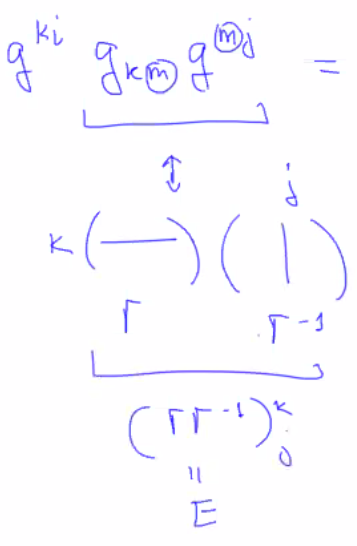
\includegraphics[width=100px]{pic16}
	\end{proof}
	\textbf{Отступление:}\n
	$\begin{matrix}
		e_1 \ldots d_n\\
		e'_1 \ldots e'_n
	\end{matrix}$ базисы $V$\n
	Говорят, что базисы принадлежат одному классу ориентации, если $det T_{e\rightarrow e'} > 0$\n
	В $\forall$ пространстве $\exists$ 2 класса ориентации на плоскости:
	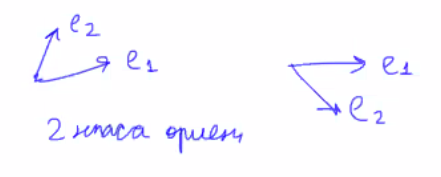
\includegraphics[width=180px]{pic17} \n в пространстве: $\begin{matrix}
		\text{правая тройка}\\
		\text{левая тройка}
	\end{matrix}$\n
	В нашем случае, \underline{взаимные базисы} всегда $\in$ \underline{одному классу ориентации},\n
	т.к. $T_{e_i \rightarrow e^j} = \Gamma^{-1} = G(e^1 \ldots e^n) > 0$
	\begin{corollary}
	$e_1 \ldots e_n$ о.н.б. $V \Rightarrow \underset{\text{взаимные совпадают с исходными}}{e^i = e_i \; \; \; \forall i = 1\ldots n}$
	\end{corollary}
	\begin{proof}
		$e$ о.н.б. $\Rightarrow G(e_1 \ldots e_n) = E = \Gamma \Rightarrow \Gamma^{-1} = E = T_{e_i \rightarrow e^j} \Rightarrow e^i = e_i$
	\end{proof}
	\begin{theorem}
		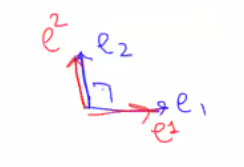
\includegraphics[width=100px]{pic18}\n
		$V \cong V^*$ из Теоремы Рисса ($\forall y \in V \leftrightarrow f \in V^*: \forall x \in V \; f(x) = (x, y)$)\n
		$e_1 \ldots e_n$ базис $V\n
		w^1 \ldots w^n$ сопряженный базис $V^*\n
		V^* \ni \omega^i \underset{\text{изоморф.}}{\leftrightarrow} e^i \in V \; \Rightarrow e^i$ взаимные базисы к $e_j$
	\end{theorem}
	Тут я не успел, надо повторить\\
	\begin{examples}\ \\
		$e_1 = \begin{pmatrix}
			2\\6\\5
		\end{pmatrix} \; e_2 = \begin{pmatrix}
			5\\3\\-2
		\end{pmatrix} \; e_3 = \begin{pmatrix}
			7\\4\\-3
		\end{pmatrix} \; \; \; 
			\text{Найти взаимный базис!}$\n
		Координаты $e_i$ заданы относительно о.н.б. $(x, y) = \sum\limits_{i=1}^n x^i y^i$\n
		\textbf{1 сп.} $\Gamma = G(e_1, e_2, e_3) = \begin{pmatrix}
			65 & 18 & 23\\
			18 & 38 & 53\\
			23 & 53 & 74
		\end{pmatrix}\n
		(e^1 e^2 e^3) = (e_1 e_2 e_3) \Gamma^{-1}\n
		(e^1 e^2 e^3) = \begin{pmatrix}
			2 & 5 & 7\\
			6 & 3 & 4\\
			5 & -2 & 3
		\end{pmatrix} 
		\underbracket{\begin{pmatrix}
			65 & 17 & 23\\
			18 & 38 & 53\\
			23 & 53 & 74
		\end{pmatrix}^{-1}}_{\begin{matrix}
			\begin{pmatrix}
				3 & -113 & 80\\
				-113 & 4201 & -3031\\
				80 & -3031 & 2146
			\end{pmatrix}\\
			e^1 \; e^2 \; e^3 \text{ координаты базиса}\\ \text{относительно ... не допписал}
		\end{matrix}} = \begin{matrix}
			e^1 \; e^2 \; e^3 \; \leftarrow \text{координаты векторов взаимного}\\ \text{базиса в исходном о.н.б.}\\
			\begin{pmatrix}
				1 & -38 & 27\\
				-1 & 41 & -29\\
				1 & -34 & 24
			\end{pmatrix}
		\end{matrix}$\n
		\textbf{2 сп.}\n
		$\omega^1 \omega^2 \omega^3$ сопряж. к $e_1 e_2 e_3\n
		\begin{pmatrix}
			\omega^1\\\omega^2 \\\omega^3
		\end{pmatrix} \begin{pmatrix}
			e_1 & e_2 & e_3
		\end{pmatrix} = E \Rightarrow \begin{pmatrix}
			\omega^1\\\omega^2\\\omega^3
		\end{pmatrix} = \begin{pmatrix}
			2&5&7\\6&3&4\\5&-2&-3
		\end{pmatrix}^{-1} = \begin{pmatrix}
			1&-1&1\\-38&41&-34\\27&-29&24
		\end{pmatrix} \begin{matrix}
			\rightarrow \omega^1\\
			\rightarrow \omega^2\\
			\rightarrow \omega^3
		\end{matrix}$\n
		По теореме 2: $(\R^3)^* \equiv \R_3 \underset{\text{изоморф. т-ма 2}}{\cong} \R^3\n
		\omega^i \leftrightarrow e^i\\
		\omega^i (x) = (x, e^i)\n
		e^1 = \begin{pmatrix}
			1\\-1\\1
		\end{pmatrix} \; e^2 = \begin{pmatrix}
			-38\\41\\-34
		\end{pmatrix} \; e^3 = \begin{pmatrix}
			27\\-29\\24
		\end{pmatrix}$
	\end{examples}
	\begin{defin}
		$e^i$ и $e_j$ взаимные базисы $V$\n
		$\forall x \in V \; \; x = x^i e_i = x_j e^j\n
		x^i$ -- \underline{контрвариант.} координаты вектора\\
		$x_j$ -- \underline{ковариант.} координаты вектора\n
		$e^j \leftrightarrow \underset{\text{сопряж. к }e_i}{\omega^j \in V^*}\n
		\boxed{\begin{matrix}
				x^i = \omega^i (x) = (x, e^i)\\
				x_j = e_j(x) = (x, e_j)
			\end{matrix}}$
	\end{defin}
	$T = T_{e\rightarrow e'} \; \; S = T^{-1} \; \; \; \; \; \; \boxed{\begin{matrix}x'^i = s^i_j x^j\\
	x'_j = t^i_j x_i\end{matrix}}\n
	\begin{matrix}
		e_1 \ldots e_n\\e^1 \ldots e^n
	\end{matrix} \; \begin{matrix}
		e'_1 \ldots e'_n\\e'^1 \ldots e'^n
	\end{matrix}\n
	\boxed{\begin{matrix}
			x = x^i e_i = (x, e^i) e_i\\
			x = x_j e^j = (x, e_j) e^j
		\end{matrix}}$ формулы Гибса\n
	\begin{defin}
		$\begin{matrix}
			(x^i) \text{ контрвар. координаты вектора } x \text{ -- тензор типа } (0, 1)\n
			(x_j) \text{ ковар. координаты вектора } x \text{ -- тензор типа } (1, 0)
		\end{matrix}$\n
		\underline{Сверткой} этих \underline{тензоров} с \underline{метрическими тензорами $\Gamma$ и $\Gamma^{-1}$}, соответственно, называются следующие операции:\\
		$\boxed{g_{ji} x^i = g_{ij} x^i}$ и $\boxed{g^{ij} x_i = g^{ji} x_i}$ ($\Leftrightarrow$ свертка произв. тензоров)\n
		$\boxed{\begin{matrix}
			g_{ij} x^i = g_{ij} (x, e^i) = (x, g_{ij} e^i) = (x, e_j) = x_j\n
			g^{ij} x_i = g^{ij} (x, e_i) = (x, g^{ij} e_i) = (x, e^j) = x^J
			\end{matrix}}
		$ \underline{операции поднятия и опускания индекса тензора}
	\end{defin}
	\begin{examples}
		$\forall x, y \in V \slide{20px} (x, y) = \underbracket{g_{ij} x^i}_{x_j} y^j = x_j \underset{\stackrel{||}{ \underbracket{g^{ij} y_i}}}{y^j} = g^{ij} x_j y_i = \xi^T \Gamma^{-1} \eta = (x,y)\n
		\begin{matrix}
			x^T \Gamma y\\
			\Gamma = G(e_1 \ldots e_n)\\
			x = x^i e_i\\
			y = y^j e_j
		\end{matrix} \slide{30px} \begin{matrix}
			\Gamma^{-1} = G(e^1 \ldots e^n)\\
			\xi = (\xi_1 \ldots \xi_n)\\
			x = \xi_i e^i\\
			y = \eta_j e^j
		\end{matrix}$
	\end{examples}
	$V$ Евклидово пространство, $\Gamma, \Gamma^{-1}$ метр. тензоры.
	\begin{defin}
		$\alpha \in T(p, q) \; \; q\geq 1$ \underline{опусканием верхнего индекса} тензора $\alpha$
		называется его свертка с ковариантн. метр. тензором ($\Gamma$) по тому
		верхнему индексу, который следует опустить. В результате, получаем тензор $\in T_{(p+1, q-1)}$
	\end{defin}
	\begin{defin}
		$\alpha \in T(p, q) \ \; p\geq 1$ \underline{поднятием нижнего индекса} $\alpha$ называется
		его свертка с контрвариантн. метр. тензором ($\Gamma^{-1}$) по тому нижнему индексу, который следует поднять. В результате, получаем тензор $\in T(p-1, q+1)$
	\end{defin}
	\underline{При опускании верхнего индекса} он всегда записывается нижними левым. Если опускаются несколько индексов, то они записываются в том же порядке, в котором стояли сверху.\n
	\underline{При поднятии нижнего индекса} он всегда записывается правым верхним. Если поднимаются несколько индексов, то они записываются в том же порядке, в котором стояли внизу.\n
	$g_{j_0 s} \alpha^{i_1 \ldots i_{q-1} s}_{j_1 \ldots j_p} \in T(p, q) = \alpha^{i_1 \ldots i_{q-1}}_{j_0 j_1 \ldots j_p} \in T(p+1, q-1) $ 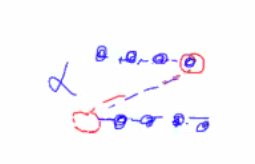
\includegraphics[width=100px]{pic19} \n
	$g^{s i_{q+1}} \alpha_{s j_2 \ldots j_p}^{j_1 \ldots j_q} \in T(p, q)= \alpha^{i_1 \ldots i_q i_{q+1}}_{j_2 \ldots j_p} \in T(p-1, q+1)$\n
	Стандартный порядок следования индексов (сначала верхние, потом нижние)\\
	В остальных случаях, дополнительно прежнее место индекса отмечается точкой.\n
	Например, $\begin{matrix}g_{is} \alpha^{sj}_k = \alpha^{\cdot j}_{ik}\\
	g^{sk} \alpha^i_{js} = \alpha^{ik}_{j\cdot}\end{matrix}\n
	g_{is} g_{kr} \alpha^{sjrl}_m = \alpha^{\cdot j \cdot l}_{ikm} \; \; \begin{matrix}
		i \text{ стр}\\
		j \text{ стол.}\\
		k \text{ слой}\\
		l \text{ срез}\\
		m \text{ след. слой}
	\end{matrix}\n
	\alpha^{\cdot 3 \cdot 1}_{2 4 2} \begin{matrix}
		\text{тут не успел}
	\end{matrix}$
	\begin{examples}
		\begin{mylist}\
			\item 
			$\alpha \in T(2, 0) \leftrightarrow A = \begin{pmatrix}
				0 & 1 & 3\\
				2 & 3 & 5\\
				3 & 5 & 7
			\end{pmatrix}\n
			\Gamma = \begin{pmatrix}
				21 & -10 & -4\\
				-10 & 5 & 2\\
				-4 & 2 & 1
			\end{pmatrix} = (g_{ij})$\n
			\begin{mylist}
				\item найти матрицу тензора с поднятым 1-м индексом
				\item ... с 2-м индексом
				\item ... с 2-мя индексами
			\end{mylist}
			$\Gamma^{-1} = (g^{ij}) = \begin{pmatrix}
				1 & 2 & 0\\
				2 & 5 & -2\\
				0 & -2 & 5
			\end{pmatrix}$
			\begin{mylist}
				\item 
				$\alpha_{ij} \leadsto \alpha_j^i = g^{\stackrel{\boxed{ik}}{ki}} \alpha _{kj} = g^{ik} \alpha_{kj} \leftrightarrow \Gamma^{-1} A$\n
				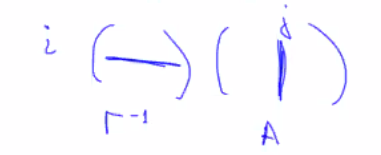
\includegraphics[width=100px]{pic20}\n
				$(\alpha^i_j) = \Gamma^{-1} A = \begin{pmatrix}
					4 & 7 & 13\\
					4 & 7 & 17\\
					11 & 9 & 25
				\end{pmatrix}$
				\item 
				$\alpha_{ij} \leadsto \alpha^j_{i\cdot} = g^{\stackrel{jk}{\boxed{kj}}} \alpha_{ik}
				 = \alpha_{ik} g^{kj} \leftrightarrow A \Gamma^{-1} \; \; \; \; (\alpha^j_{i\cdot}) = A \Gamma^{-1} = \begin{pmatrix}
					 2 & -1 & 13\\
					 8 & 9 & 19\\
					 13 & 7 & 25
				 \end{pmatrix}$\n
				 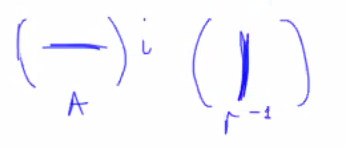
\includegraphics[width=100px]{pic21} 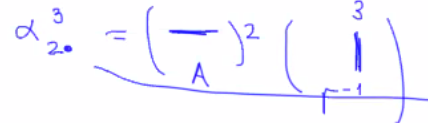
\includegraphics[width=130px]{pic22}
				 \item 
				 $\alpha_{ij} \leadsto \alpha^{ij} = g^{ik} g^{mj} \alpha_{km} \leftrightarrow \Gamma^{-1} A \Gamma^{-1}\n
				 (\alpha^{ij}) = \begin{pmatrix}
					 18 & 17 & 51\\
					 18 & 9 & 71\\
					 49 & 69 & 87
				 \end{pmatrix}$
			\end{mylist}
			\item 
			$\alpha \in T(2, 1) \; \; \Gamma $ ... не дописал\n
			$\alpha^i_{jk} \; \; \; \; A = \begin{matrix}
				\left(\begin{array}{ccc}
					0 & -1 & 1\\1 & 0 & -1\\-1 & 1 & 0
				\end{array}\right| & \left.\begin{array}{ccc}
					0 & 2 & -2\\-2 & 0 & 2\\2 & -2 & 0
				\end{array}\right| & \left.\begin{array}{ccc}
					0 & -1 & 1\\1 & 0 & -1\\ -1 & 1 & 0
				\end{array}\right)\\
				A_1 & A_2 & A_3
			\end{matrix}$
			\begin{mylist}
				\item 
					$\alpha^i_{jk} \leadsto \alpha_{ijk} = g_{im} \alpha^m_{jk} = (\Gamma A_k)^i_j$ 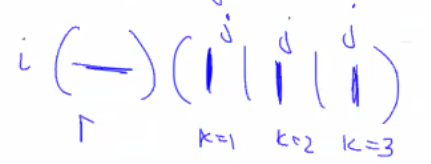
\includegraphics[width=120px]{pic23}\n
					$(\alpha_{ijk}) = (\Gamma A_1 | \Gamma A_2 | \Gamma A_3) = \begin{pmatrix}
						\text{Сами посчитаете}
					\end{pmatrix}$
				\item
				$\alpha^i_{jk} \leadsto \alpha^{ik}_{j\cdot} = g^{mk} \alpha^i_{jm} = \alpha^i_{j1} g^{1k} + \alpha^i_{j2} g^{2k} + \alpha^i_{j3} g^{3k} = \\
				= 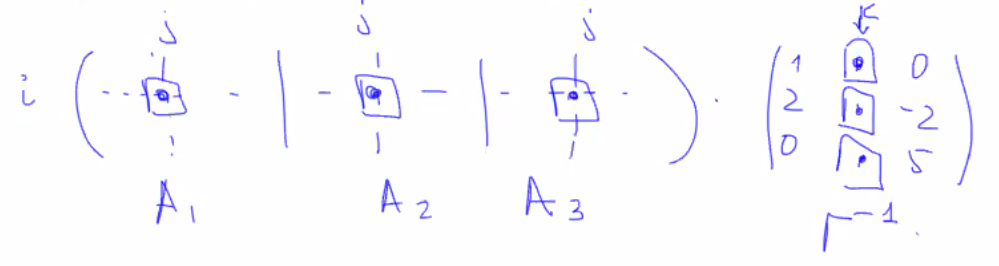
\includegraphics[width=380px]{pic24} = \n
				= \begin{pmatrix}
					1\cdot A_1 + 2A_2 + 0A_3 & | 2A_1 + 5A_2 - 2A_3 & | 0A_1 - 2A_2 + 5A_3\\
					k = 1 & k=2 & k = 3
				\end{pmatrix} = \begin{pmatrix}
					\text{Опять сами(}
				\end{pmatrix}$
			\end{mylist}
		\end{mylist}
	\end{examples}
	$\pu$ о.н.б. $V \; \; \; \; \Gamma = E = \Gamma^{-1} \Rightarrow$ все тензоры, которые получены сверткой с такими метр. тензорами будут отличаться друг от друга только расположением верхних и нижних индексов.\n
	Например, $\alpha^{\cdot j}_{ik} = \underset{=\delta_{is}}{g_{is}} \alpha^{si}_k = \alpha_k^{ij}\; \; \; $ Элементы в обеих матрицах одинаковые.\n
	$e, e'$ о.н.б. $V\n
	T = \underset{\text{ортог.}\rightarrow}{T_{e\rightarrow e'}} \boxed{T^{-1} = S = T^T}\n$
	\Large$$\alpha'^{i_1' \ldots i_q'}_{j_1' \ldots j_p'} = \alpha^{i_1 \ldots i_q}_{j_1 \ldots j_p} t^{j_1}_{j_1'} \ldots t^{j_p}_{j_p'} s^{i_1'}_{i_1} \ldots s^{i'_q}_{iq} = 
	\sum\limits_{i_1=1}^n \ldots \sum\limits_{i_q = 1}^n \alpha^{i_1 \ldots i_q}_{j_1 \ldots j_p} t^{j_1}_{j_1'} \ldots t^{i_p}_{i_p'} \ldots t^{i_q}_{i'_q}$$
	\normalsize
	\begin{defin}
		Все тензоры, которые после преобразования к \underline{одному} о.н.б. \underline{евкл. пр-ва}, отличающиеся только расположением верхних и нижних индексов, считаем равными и \\называем \underline{евклидовыми тензорами}.\n
		$\underset{\stackrel{||}{p+q}}{r \text{ -- валентность}} \; \; \; \; \alpha_{i_1 \ldots i_p j_1 \ldots j_q} \; \; \; \; \; \; \; T(p, q) \leftrightarrow \text{ определяет }(p+q) \text{ евкл. тензор}\n
		\boxed{\alpha'_{i_1' \ldots i'_r} = \alpha_{i_1 \ldots i_r} t^{i_1}_{i_1'} \ldots t^{i_r}_{i'_r}}$
	\end{defin}
\end{document}